\providecommand{\qcOne}{\mathbf{1}}   %
\providecommand{\qcTwo}{\mathbf{2}}   %
\providecommand{\qcor}[1]{\ulcorner#1\urcorner}   %
\providecommand{\Cat}{\mathcal{C}at}
\providecommand{\QCat}{\mathcal{Q}\mathcal{C}at}

\section{逗号构造}\label{sec:the-comma-construction}

\textbf{\trCommaInfinityCategory}（comma ∞-category）定义为：沿一对余定义域为 $A$ 的%
指定函子，限制\trArrowInfinityCategory{} $A^{2}$ 的定义域与余定义域。

\begin{definition}[\trCommaInfinityCategory]\label{def:comma-infinity-category}
设 $C\xrightarrow{\;g\;}A\xleftarrow{\;f\;}B$ 是由\trInfinityCategory{}构成的%
一个\trDiagram{}。\textbf{\trCommaInfinityCategory}定义为\trSimplicial\trCotensor{} $A^{2}$%
沿 $g\times f$ 的一个\trPullback
\begin{rveq}\label{eq:comma-pullback}
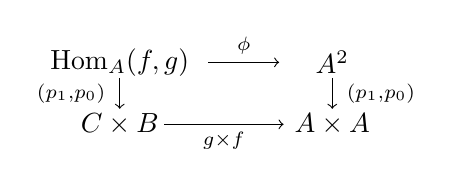
\begin{tikzpicture}[x=1.6em,y=1.6em,baseline=(current bounding box.center)]
  \node (tl) at (0,1.4) {$\mathrm{Hom}_A(f,g)$};
  \node (tr) at (4.8,1.4) {$A^{2}$};
  \node (bl) at (0,0) {$C\times B$};
  \node (br) at (4.8,0) {$A\times A$};
  \draw[->] (2.0,1.4) -- (3.6,1.4);
  \node at (2.8,1.78) {$\scriptstyle\qcor{\phi}$};
  \draw[->] (0,1.05) -- (0,0.35);
  \node at (-1.1,0.7) {$\scriptstyle(p_{1},p_{0})$};
  \node at (0.48,0.78) {$\scriptstyle\lrcorner$};
  \draw[->] (4.8,1.05) -- (4.8,0.35);
  \node at (5.9,0.7) {$\scriptstyle(p_{1},p_{0})$};
  \draw[->] (1.0,0) -- (3.7,0);
  \node at (2.35,-0.36) {$\scriptstyle g\times f$};
\end{tikzpicture}
\end{rveq}
这一构造为\trCommaInfinityCategory{}配备了一个指定的\trIsofibration{}%
$(p_{1},p_{0})\colon\mathrm{Hom}_A(f,g)\twoheadrightarrow C\times B$，以及%
\trHomotopyTwoCategory{}中的一个典范\trNaturalTransformation
\begin{rveq}\label{eq:comma-cone}
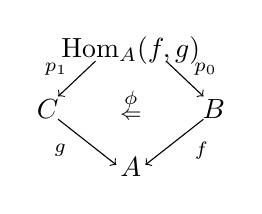
\begin{tikzpicture}[x=1.5em,y=1.5em,baseline=(current bounding box.center)]
  \node (hom) at (0,2.2) {$\mathrm{Hom}_A(f,g)$};
  \node (c) at (-2.0,0.8) {$C$};
  \node (b) at (2.0,0.8) {$B$};
  \node (a) at (0,-0.6) {$A$};
  \draw[->] (-0.85,1.95) -- (-1.75,1.1);
  \node at (-1.8,1.75) {$\scriptstyle p_{1}$};
  \draw[->] (0.85,1.95) -- (1.75,1.1);
  \node at (1.8,1.75) {$\scriptstyle p_{0}$};
  \node at (0,1.02) {$\scriptstyle\phi$};
  \node at (0,0.64) {$\scriptstyle\Leftarrow$};
  \draw[->] (-1.75,0.55) -- (-0.35,-0.55);
  \node at (-1.7,-0.2) {$\scriptstyle g$};
  \draw[->] (1.75,0.55) -- (0.35,-0.55);
  \node at (1.7,-0.2) {$\scriptstyle f$};
\end{tikzpicture}
\end{rveq}
后者称为\textbf{\trCommaCone}（comma cone）。
\end{definition}

由 \eqref{eq:comma-pullback} 的\trUniversalProperty{}，\trCommaInfinityCategory{}的一个\trElement{}%
$(\alpha,b,c)\colon\qcOne\to\mathrm{Hom}_A(f,g)$ 是一个三元组，其中 $b$ 与 $c$ 分别%
是 $B$ 与 $C$ 的\trElement{}，而 $\alpha\colon fb\to gc$ 是 $A$ 中一条以 $fb$ 为定义域、%
以 $gc$ 为余定义域的箭头。

\begin{example}\label{exa:arrows-as-comma}
\trArrowInfinityCategory{}作为应用于恒同\trSpan{}（identity span）的逗号构造的特例而出现。%
这为 \eqref{eq:generic-arrow} 的\trGenericArrow{}提供了另一种记号
\begin{center}
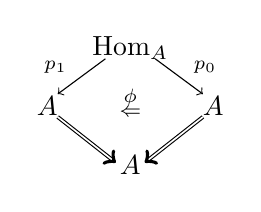
\begin{tikzpicture}[x=1.5em,y=1.5em]
  \node (hom) at (0,2.2) {$\mathrm{Hom}_A$};
  \node (al) at (-2.0,0.8) {$A$};
  \node (ar) at (2.0,0.8) {$A$};
  \node (ab) at (0,-0.6) {$A$};
  \draw[->] (-0.6,1.95) -- (-1.75,1.1);
  \node at (-1.8,1.75) {$\scriptstyle p_{1}$};
  \draw[->] (0.6,1.95) -- (1.75,1.1);
  \node at (1.8,1.75) {$\scriptstyle p_{0}$};
  \node at (0,1.02) {$\scriptstyle\phi$};
  \node at (0,0.64) {$\scriptstyle\Leftarrow$};
  \draw[double,->] (-1.75,0.55) -- (-0.35,-0.55);
  \draw[double,->] (1.75,0.55) -- (0.35,-0.55);
\end{tikzpicture}
\end{center}
它可视为\trCommaCone{}的一个特例。
\end{example}

下列命题编码了逗号构造的诸\trHomotopy{}论性质。

\begin{proposition}[逗号之间的映射]\label{prop:maps-between-commas}
交换\trDiagram
\begin{center}
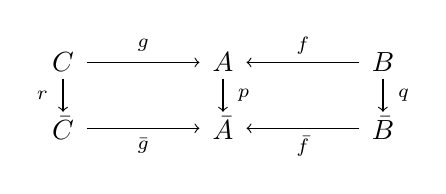
\begin{tikzpicture}[x=1.7em,y=1.7em]
  \node (c) at (0,1.4) {$C$};
  \node (a) at (3.4,1.4) {$A$};
  \node (b) at (6.8,1.4) {$B$};
  \node (cb) at (0,0) {$\bar{C}$};
  \node (ab) at (3.4,0) {$\bar{A}$};
  \node (bb) at (6.8,0) {$\bar{B}$};
  \draw[->] (0.5,1.4) -- (2.9,1.4);
  \node at (1.7,1.76) {$\scriptstyle g$};
  \draw[->] (6.3,1.4) -- (3.9,1.4);
  \node at (5.1,1.76) {$\scriptstyle f$};
  \draw[->] (0.5,0) -- (2.9,0);
  \node at (1.7,-0.38) {$\scriptstyle\bar{g}$};
  \draw[->] (6.3,0) -- (3.9,0);
  \node at (5.1,-0.38) {$\scriptstyle\bar{f}$};
  \draw[->] (0,1.05) -- (0,0.35);
  \node at (-0.44,0.7) {$\scriptstyle r$};
  \draw[->] (3.4,1.05) -- (3.4,0.35);
  \node at (3.84,0.7) {$\scriptstyle p$};
  \draw[->] (6.8,1.05) -- (6.8,0.35);
  \node at (7.24,0.7) {$\scriptstyle q$};
\end{tikzpicture}
\end{center}
诱导出\trCommaInfinityCategory{}之间的一个映射
\begin{center}
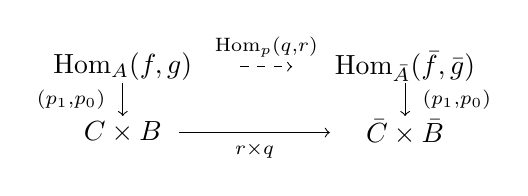
\begin{tikzpicture}[x=1.7em,y=1.7em]
  \node (tl) at (0,1.4) {$\mathrm{Hom}_A(f,g)$};
  \node (tr) at (6.0,1.4) {$\mathrm{Hom}_{\bar{A}}(\bar{f},\bar{g})$};
  \node (bl) at (0,0) {$C\times B$};
  \node (br) at (6.0,0) {$\bar{C}\times\bar{B}$};
  \draw[->,dashed] (2.5,1.4) -- (3.6,1.4);
  \node at (3.05,1.82) {$\scriptstyle\mathrm{Hom}_p(q,r)$};
  \draw[->] (0,1.05) -- (0,0.35);
  \node at (-1.1,0.7) {$\scriptstyle(p_{1},p_{0})$};
  \draw[->] (6.0,1.05) -- (6.0,0.35);
  \node at (7.1,0.7) {$\scriptstyle(p_{1},p_{0})$};
  \draw[->] (1.2,0) -- (4.4,0);
  \node at (2.8,-0.38) {$\scriptstyle r\times q$};
\end{tikzpicture}
\end{center}
此外，若 $p$、$q$ 与 $r$ 全为\trIsofibration{}、全为\trTrivialFibration{}或全为%
\trEquivalence{}，则诱导映射也相应地仍为\trIsofibration{}、\trTrivialFibration{}或%
\trEquivalence{}。
\end{proposition}

\begin{proof}
\trCospan{}之映射给出如下交换\trDiagram
\begin{center}
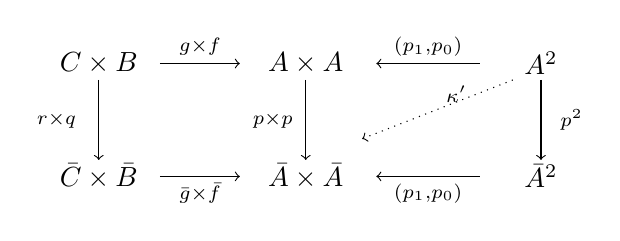
\begin{tikzpicture}[x=1.7em,y=1.7em]
  \node (tl) at (0,1.7) {$C\times B$};
  \node (tm) at (4.4,1.7) {$A\times A$};
  \node (tr) at (9.4,1.7) {$A^{2}$};
  \node (bl) at (0,-0.7) {$\bar{C}\times\bar{B}$};
  \node (bm) at (4.4,-0.7) {$\bar{A}\times\bar{A}$};
  \node (br) at (9.4,-0.7) {$\bar{A}^{2}$};
  \draw[->] (1.3,1.7) -- (3.0,1.7);
  \node at (2.15,2.06) {$\scriptstyle g\times f$};
  \draw[->] (8.1,1.7) -- (5.9,1.7);
  \node at (7.0,2.06) {$\scriptstyle(p_{1},p_{0})$};
  \draw[->] (1.3,-0.7) -- (3.0,-0.7);
  \node at (2.15,-1.06) {$\scriptstyle\bar{g}\times\bar{f}$};
  \draw[->] (8.1,-0.7) -- (5.9,-0.7);
  \node at (7.0,-1.06) {$\scriptstyle(p_{1},p_{0})$};
  \draw[->] (0,1.35) -- (0,-0.35);
  \node at (-0.9,0.5) {$\scriptstyle r\times q$};
  \draw[->] (4.4,1.35) -- (4.4,-0.35);
  \node at (3.7,0.5) {$\scriptstyle p\times p$};
  \draw[->] (9.4,1.35) -- (9.4,-0.35);
  \node at (10.05,0.5) {$\scriptstyle p^{2}$};
  \draw[->,dotted] (8.8,1.35) -- (5.6,0.1);
  \node at (7.6,1.05) {$\scriptstyle\kappa'$};
  \node at (5.95,0.42) {$\scriptstyle\lrcorner$};
\end{tikzpicture}
\end{center}
其中点线映射是\trMonomorphism{} $\qcOne+\qcOne\hookrightarrow\qcTwo$ 与 $p$ 的 \trLeibnizTensor{}。%
若 $p$、$q$ 与 $r$ 是\trIsofibration{}或\trTrivialFibration{}，则据第 1 章中的%
定义 1.2.1(ii) 与引理 1.2.14，此映射与其余四个向下的映射也相应地全是%
\trIsofibration{}或\trTrivialFibration{}。
由附录 C 中的命题 C.1.12，映射 $\mathrm{Hom}_p(q,r)$ 仍是\trIsofibration{}或%
\trTrivialFibration{}（见\cref{ex:hom-p-factors}）。
在 $p$、$q$ 与 $r$ 为\trEquivalence{}的情形，引理 1.2.15 蕴含 $r\times q$、$p\times p$%
与 $p^{2}$ 亦然，于是命题 3.3.4 适用，证得 $\mathrm{Hom}_p(q,r)$ 是一个\trEquivalence{}。
\end{proof}

存在一个与\cref{def:comma-infinity-category}相类比的 2-范畴论\trLimit{}概念：它构造%
居于一个指定\trCospan{}之上的方形中的泛 2-\trCell{}。在 $\Cat$ 中，这一\trUniversalProperty{}%
刻画了\textbf{\trCommaCategory}（comma category）——「逗号」之名即借自于此。%
与\trArrowInfinityCategory{}的情形一样，\trCommaInfinityCategory{}并\emph{不}严格满足%
这一 2 维\trUniversalProperty{}。取而代之的有：

\begin{proposition}[\trCommaInfinityCategory{}的弱\trUniversalProperty]\label{prop:comma-weak-universal-property}
\trCommaCone \eqref{eq:comma-cone} 在\trHomotopyTwoCategory{}中具有由下述三种运算给出的%
弱\trUniversalProperty{}：
\begin{enumerate}[label=(\roman*)]
\item \textbf{\trOneCellInduction{}：}给定\trCospan{} $C\xrightarrow{\;g\;}A\xleftarrow{\;f\;}B$%
之上的一个\trNaturalTransformation{}，如下左图所示：
\begin{center}
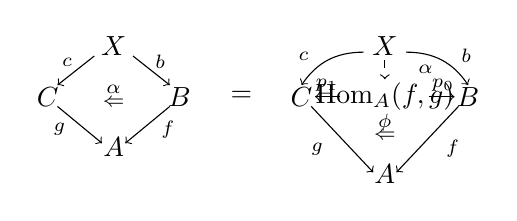
\begin{tikzpicture}[x=1.4em,y=1.4em]
  \node (x) at (0,2.6) {$X$};
  \node (c) at (-1.7,1.3) {$C$};
  \node (b) at (1.7,1.3) {$B$};
  \node (a) at (0,0) {$A$};
  \draw[->] (-0.5,2.35) -- (-1.45,1.6);
  \node at (-1.2,2.2) {$\scriptstyle c$};
  \draw[->] (0.5,2.35) -- (1.45,1.6);
  \node at (1.2,2.2) {$\scriptstyle b$};
  \node at (0,1.5) {$\scriptstyle\alpha$};
  \node at (0,1.14) {$\scriptstyle\Leftarrow$};
  \draw[->] (-1.45,1.05) -- (-0.3,0.1);
  \node at (-1.4,0.45) {$\scriptstyle g$};
  \draw[->] (1.45,1.05) -- (0.3,0.1);
  \node at (1.4,0.45) {$\scriptstyle f$};
  \node at (3.3,1.3) {$=$};
  \begin{scope}[shift={(7.0,0)}]
  \node (x) at (0,2.6) {$X$};
  \node (hom) at (0,1.3) {$\mathrm{Hom}_A(f,g)$};
  \draw[->,dashed] (0,2.25) -- (0,1.75);
  \node at (1.05,2.0) {$\scriptstyle\qcor{\alpha}$};
  \draw[->] (-0.55,2.45) to[bend right=28] (-2.15,1.6);
  \node at (-2.1,2.35) {$\scriptstyle c$};
  \draw[->] (0.55,2.45) to[bend left=28] (2.15,1.6);
  \node at (2.1,2.35) {$\scriptstyle b$};
  \node (c) at (-2.15,1.3) {$C$};
  \node (b) at (2.15,1.3) {$B$};
  \draw[->] (-1.15,1.3) -- (-1.8,1.3);
  \node at (-1.5,1.6) {$\scriptstyle p_{1}$};
  \draw[->] (1.15,1.3) -- (1.8,1.3);
  \node at (1.5,1.6) {$\scriptstyle p_{0}$};
  \node at (0,0.62) {$\scriptstyle\phi$};
  \node at (0,0.3) {$\scriptstyle\Leftarrow$};
  \node (a) at (0,-0.7) {$A$};
  \draw[->] (-1.9,1.05) -- (-0.3,-0.65);
  \node at (-1.75,-0.05) {$\scriptstyle g$};
  \draw[->] (1.9,1.05) -- (0.3,-0.65);
  \node at (1.75,-0.05) {$\scriptstyle f$};
  \end{scope}
\end{tikzpicture}
\end{center}
则存在\trFunctor{} $\qcor{\alpha}\colon X\to\mathrm{Hom}_A(f,g)$，使得 $b=p_{0}\qcor{\alpha}$、%
$c=p_{1}\qcor{\alpha}$，且 $\alpha=\phi\qcor{\alpha}$。
\item \textbf{\trTwoCellInduction{}：}给定\trFunctor{} $a,a'\colon X\to\mathrm{Hom}_A(f,g)$%
与\trNaturalTransformation{} $\tau_{1}$、$\tau_{0}$，使得
\begin{center}
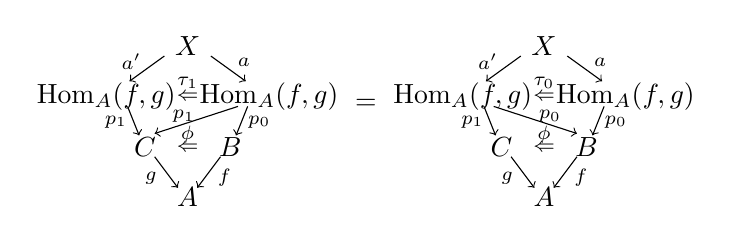
\begin{tikzpicture}[x=1.4em,y=1.4em]
  \node (x) at (0,2.8) {$X$};
  \node (hl) at (-2.1,1.5) {$\mathrm{Hom}_A(f,g)$};
  \node (hr) at (2.1,1.5) {$\mathrm{Hom}_A(f,g)$};
  \draw[->] (-0.6,2.55) -- (-1.5,1.9);
  \node at (-1.45,2.4) {$\scriptstyle a'$};
  \draw[->] (0.6,2.55) -- (1.5,1.9);
  \node at (1.45,2.4) {$\scriptstyle a$};
  \node at (0,1.85) {$\scriptstyle\tau_{1}$};
  \node at (0,1.5) {$\scriptstyle\Leftarrow$};
  \node (c) at (-1.1,0.2) {$C$};
  \node (b) at (1.1,0.2) {$B$};
  \draw[->] (-1.55,1.25) -- (-1.25,0.5);
  \node at (-1.85,0.85) {$\scriptstyle p_{1}$};
  \draw[->] (1.55,1.25) -- (1.25,0.5);
  \node at (1.85,0.85) {$\scriptstyle p_{0}$};
  \draw[->] (1.3,1.25) -- (-0.85,0.55);
  \node at (-0.1,1.0) {$\scriptstyle p_{1}$};
  \node at (0,0.52) {$\scriptstyle\phi$};
  \node at (0,0.18) {$\scriptstyle\Leftarrow$};
  \node (a2) at (0,-1.1) {$A$};
  \draw[->] (-0.85,-0.05) -- (-0.25,-0.85);
  \node at (-0.95,-0.6) {$\scriptstyle g$};
  \draw[->] (0.85,-0.05) -- (0.25,-0.85);
  \node at (0.95,-0.6) {$\scriptstyle f$};
  \node at (4.6,1.3) {$=$};
  \begin{scope}[shift={(9.2,0)}]
  \node (x) at (0,2.8) {$X$};
  \node (hl) at (-2.1,1.5) {$\mathrm{Hom}_A(f,g)$};
  \node (hr) at (2.1,1.5) {$\mathrm{Hom}_A(f,g)$};
  \draw[->] (-0.6,2.55) -- (-1.5,1.9);
  \node at (-1.45,2.4) {$\scriptstyle a'$};
  \draw[->] (0.6,2.55) -- (1.5,1.9);
  \node at (1.45,2.4) {$\scriptstyle a$};
  \node at (0,1.85) {$\scriptstyle\tau_{0}$};
  \node at (0,1.5) {$\scriptstyle\Leftarrow$};
  \node (c) at (-1.1,0.2) {$C$};
  \node (b) at (1.1,0.2) {$B$};
  \draw[->] (-1.55,1.25) -- (-1.25,0.5);
  \node at (-1.85,0.85) {$\scriptstyle p_{1}$};
  \draw[->] (1.55,1.25) -- (1.25,0.5);
  \node at (1.85,0.85) {$\scriptstyle p_{0}$};
  \draw[->] (-1.3,1.25) -- (0.85,0.55);
  \node at (0.15,1.0) {$\scriptstyle p_{0}$};
  \node at (0,0.52) {$\scriptstyle\phi$};
  \node at (0,0.18) {$\scriptstyle\Leftarrow$};
  \node (a2) at (0,-1.1) {$A$};
  \draw[->] (-0.85,-0.05) -- (-0.25,-0.85);
  \node at (-0.95,-0.6) {$\scriptstyle g$};
  \draw[->] (0.85,-0.05) -- (0.25,-0.85);
  \node at (0.95,-0.6) {$\scriptstyle f$};
  \end{scope}
\end{tikzpicture}
\end{center}
则存在\trNaturalTransformation{} $\tau\colon a\Rightarrow a'$，使得 $p_{1}\tau=\tau_{1}$%
且 $p_{0}\tau=\tau_{0}$。
\item \textbf{\trTwoCellConservativity{}：}对任何
\begin{center}
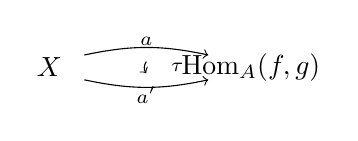
\begin{tikzpicture}[x=1.4em,y=1.4em]
  \node (x) at (0,0) {$X$};
  \node (h) at (5.2,0) {$\mathrm{Hom}_A(f,g)$};
  \draw[->] (0.9,0.32) to[bend left=12] (4.1,0.32);
  \node at (2.5,0.68) {$\scriptstyle a$};
  \draw[->] (0.9,-0.32) to[bend right=12] (4.1,-0.32);
  \node at (2.5,-0.72) {$\scriptstyle a'$};
  \draw[->] (2.5,0.15) to[bend right=35] (2.5,-0.15);
  \node at (3.3,0.0) {$\scriptstyle\tau$};
\end{tikzpicture}
\end{center}
若 $p_{1}\tau$ 与 $p_{0}\tau$ 皆为\trIsomorphism{}，则 $\tau$ 是\trIsomorphism{}。
\end{enumerate}
\end{proposition}

\begin{proof}
\trCosmologicalFunctor{} $\mathrm{Fun}(X,-)\colon\mathcal{K}\to\QCat$ 把\trPullback{}%
\eqref{eq:comma-pullback} 带为\trQuasiCategory{}的如下\trPullback
\begin{center}
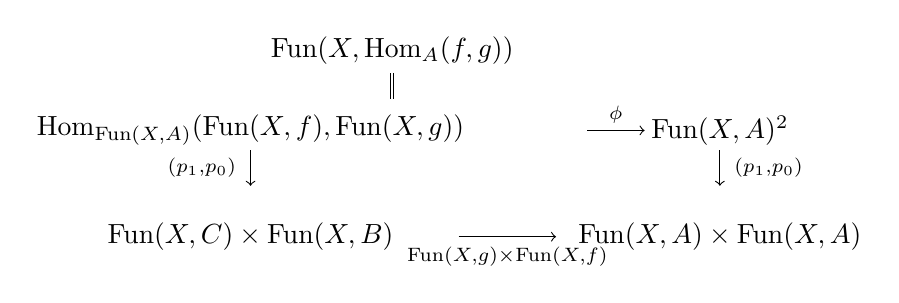
\begin{tikzpicture}[x=1.6em,y=1.6em]
  \node (top) at (3.2,3.2) {$\mathrm{Fun}(X,\mathrm{Hom}_A(f,g))$};
  \draw[double] (3.2,2.7) -- (3.2,2.1);
  \node (ml) at (0,1.4) {$\mathrm{Hom}_{\mathrm{Fun}(X,A)}(\mathrm{Fun}(X,f),\mathrm{Fun}(X,g))$};
  \node (mr) at (10.6,1.4) {$\mathrm{Fun}(X,A)^{2}$};
  \draw[->] (7.6,1.4) -- (8.9,1.4);
  \node at (8.25,1.76) {$\scriptstyle\phi$};
  \draw[->] (0,0.95) -- (0,0.15);
  \node at (-1.1,0.55) {$\scriptstyle(p_{1},p_{0})$};
  \node at (0.48,0.68) {$\scriptstyle\lrcorner$};
  \draw[->] (10.6,0.95) -- (10.6,0.15);
  \node at (11.7,0.55) {$\scriptstyle(p_{1},p_{0})$};
  \node (bl) at (0,-1.0) {$\mathrm{Fun}(X,C)\times\mathrm{Fun}(X,B)$};
  \node (br) at (10.6,-1.0) {$\mathrm{Fun}(X,A)\times\mathrm{Fun}(X,A)$};
  \draw[->] (4.7,-1.0) -- (6.9,-1.0);
  \node at (5.8,-1.44) {$\scriptstyle\mathrm{Fun}(X,g)\times\mathrm{Fun}(X,f)$};
\end{tikzpicture}
\end{center}
如今引理 3.1.7 表明：典范 2-\trCell{} \eqref{eq:comma-cone} 诱导出\trHomCategory{}之间的%
一个自然映射
\begin{center}
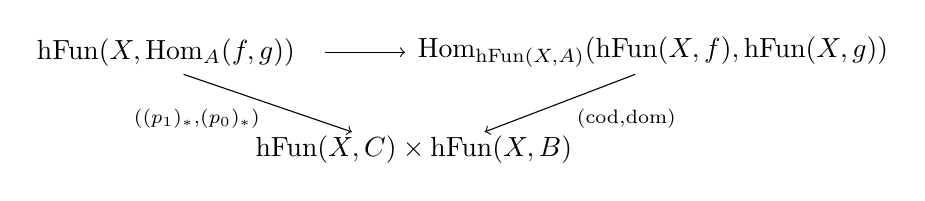
\begin{tikzpicture}[x=1.6em,y=1.6em]
  \node (tl) at (0,1.3) {$\mathrm{hFun}(X,\mathrm{Hom}_A(f,g))$};
  \node (tr) at (11.0,1.3) {$\mathrm{Hom}_{\mathrm{hFun}(X,A)}(\mathrm{hFun}(X,f),\mathrm{hFun}(X,g))$};
  \draw[->] (3.6,1.3) -- (5.4,1.3);
  \node (bm) at (5.6,-0.9) {$\mathrm{hFun}(X,C)\times\mathrm{hFun}(X,B)$};
  \draw[->] (0.4,0.8) -- (4.2,-0.5);
  \node at (0.7,-0.2) {$\scriptstyle((p_{1})_{*},(p_{0})_{*})$};
  \draw[->] (10.6,0.8) -- (7.2,-0.5);
  \node at (10.4,-0.2) {$\scriptstyle(\mathrm{cod},\mathrm{dom})$};
\end{tikzpicture}
\end{center}
它居于 $\mathrm{hFun}(X,C\times B)\cong\mathrm{hFun}(X,C)\times\mathrm{hFun}(X,B)$ 之上，%
是一个\trSmotheringFunctor{}。\trOneCellInduction{}、\trTwoCellInduction{}与%
\trTwoCellConservativity{}诸性质，分别由这一\trSmotheringFunctor{}的对象上的满射性、%
满性与保守性得证。
\end{proof}

由一个固定的\trNaturalTransformation{} $\alpha\colon fb\Rightarrow gc$ 所诱导的诸%
\trFunctor{} $\qcor{\alpha}\colon X\to\mathrm{Hom}_A(f,g)$，在 $C\times B$ 之上直至%
\trFiberedIsomorphism{}唯一。

\begin{proposition}\label{prop:whiskering-comma-bijection}
与\trCommaCone \eqref{eq:comma-cone} 作\trWhiskering{}，在下示左侧的诸\trNaturalTransformation{}%
与下示右侧的、从 $C$ 到 $B$ 的诸\trSpan{}映射的\trFiberedIsomorphism{}类之间，诱导出%
一个双射：
\[
\left\{\vcenter{\hbox{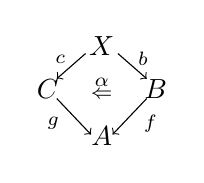
\begin{tikzpicture}[x=1.3em,y=1.3em]
  \node (x) at (0,2.2) {$X$};
  \node (c) at (-1.5,1.0) {$C$};
  \node (b) at (1.5,1.0) {$B$};
  \node (a) at (0,-0.3) {$A$};
  \draw[->] (-0.45,2.0) -- (-1.25,1.3);
  \node at (-1.15,1.85) {$\scriptstyle c$};
  \draw[->] (0.45,2.0) -- (1.25,1.3);
  \node at (1.15,1.85) {$\scriptstyle b$};
  \node at (0,1.2) {$\scriptstyle\alpha$};
  \node at (0,0.86) {$\scriptstyle\Leftarrow$};
  \draw[->] (-1.25,0.75) -- (-0.3,-0.25);
  \node at (-1.35,0.05) {$\scriptstyle g$};
  \draw[->] (1.25,0.75) -- (0.3,-0.25);
  \node at (1.35,0.05) {$\scriptstyle f$};
\end{tikzpicture}}}\right\}
\;\longleftrightarrow\;
\left\{\vcenter{\hbox{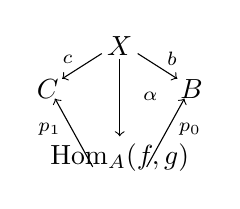
\begin{tikzpicture}[x=1.3em,y=1.3em]
  \node (x) at (0,2.6) {$X$};
  \node (c) at (-2.0,1.4) {$C$};
  \node (b) at (2.0,1.4) {$B$};
  \draw[->] (-0.5,2.4) -- (-1.6,1.7);
  \node at (-1.45,2.25) {$\scriptstyle c$};
  \draw[->] (0.5,2.4) -- (1.6,1.7);
  \node at (1.45,2.25) {$\scriptstyle b$};
  \draw[->] (0,2.25) -- (0,0.1);
  \node at (0.85,1.2) {$\scriptstyle\qcor{\alpha}$};
  \node (hom) at (0,-0.5) {$\mathrm{Hom}_A(f,g)$};
  \draw[->] (-0.75,-0.75) -- (-1.8,1.15);
  \node at (-1.95,0.3) {$\scriptstyle p_{1}$};
  \draw[->] (0.75,-0.75) -- (1.8,1.15);
  \node at (1.95,0.3) {$\scriptstyle p_{0}$};
\end{tikzpicture}}}\right\}_{/\cong}
\]
其中诸\trFiberedIsomorphism{}由\trInvertible{} 2-\trCell
\begin{center}
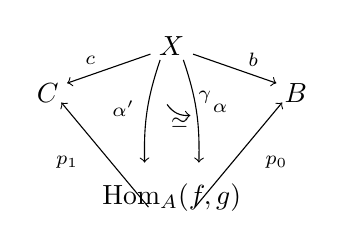
\begin{tikzpicture}[x=1.4em,y=1.4em]
  \node (x) at (0,2.4) {$X$};
  \node (c) at (-3.2,1.2) {$C$};
  \node (b) at (3.2,1.2) {$B$};
  \draw[->] (-0.55,2.2) -- (-2.7,1.45);
  \node at (-2.1,2.05) {$\scriptstyle c$};
  \draw[->] (0.55,2.2) -- (2.7,1.45);
  \node at (2.1,2.05) {$\scriptstyle b$};
  \draw[->] (-0.3,2.05) to[bend right=10] (-0.7,-0.6);
  \node at (-1.25,0.8) {$\scriptstyle\qcor{\alpha'}$};
  \draw[->] (0.3,2.05) to[bend left=10] (0.7,-0.6);
  \node at (1.25,0.8) {$\scriptstyle\qcor{\alpha}$};
  \draw[->] (-0.12,0.9) to[bend right=30] (0.48,0.62);
  \node at (0.85,1.1) {$\scriptstyle\gamma$};
  \node at (0.2,0.42) {$\scriptstyle\simeq$};
  \node (hom) at (0,-1.5) {$\mathrm{Hom}_A(f,g)$};
  \draw[->] (-0.6,-1.75) -- (-2.85,0.95);
  \node at (-2.7,-0.6) {$\scriptstyle p_{1}$};
  \draw[->] (0.6,-1.75) -- (2.85,0.95);
  \node at (2.7,-0.6) {$\scriptstyle p_{0}$};
\end{tikzpicture}
\end{center}
给出，满足 $p_{1}\gamma=\mathrm{id}_{c}$ 且 $p_{0}\gamma=\mathrm{id}_{b}$。
\end{proposition}

\begin{proof}
引理 3.1.3 证明了\cref{prop:comma-weak-universal-property}的\trSmotheringFunctor{}之%
诸\trFiber{}皆为连通\trGroupoid{}。$\alpha$ 之上的\trFiber{}，其对象是与\trCommaCone $\phi$ 作%
\trWhiskering{}后给出 $\alpha$ 的那些\trFunctor{} $X\to\mathrm{Hom}_A(f,g)$，其态射是与%
$(p_{1},p_{0})\colon\mathrm{Hom}_A(f,g)\twoheadrightarrow C\times B$ 作\trWhiskering{}后%
成为恒同 2-\trCell{} $(\mathrm{id}_{c},\mathrm{id}_{b})$ 的那些\trInvertible{}%
2-\trCell{}。\trSmotheringFunctor{}的作用在其余域的对象与各自的\trFiber{}之间定义了%
一个双射。
\end{proof}

\trHomotopyTwoCategory{}中\trCospan{}的反松弛映射同样诱导\trCommaInfinityCategory{}%
之间的映射：

\begin{observation}\label{obs:oplax-cospan-maps}
由\trOneCellInduction{}，\trDiagram
\begin{center}
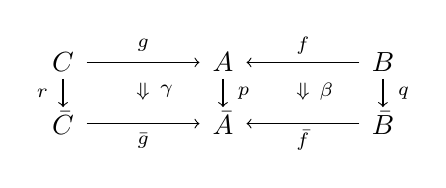
\begin{tikzpicture}[x=1.7em,y=1.7em]
  \node (c) at (0,1.3) {$C$};
  \node (a) at (3.4,1.3) {$A$};
  \node (b) at (6.8,1.3) {$B$};
  \node (cb) at (0,0) {$\bar{C}$};
  \node (ab) at (3.4,0) {$\bar{A}$};
  \node (bb) at (6.8,0) {$\bar{B}$};
  \draw[->] (0.5,1.3) -- (2.9,1.3);
  \node at (1.7,1.66) {$\scriptstyle g$};
  \draw[->] (6.3,1.3) -- (3.9,1.3);
  \node at (5.1,1.66) {$\scriptstyle f$};
  \draw[->] (0.5,0) -- (2.9,0);
  \node at (1.7,-0.36) {$\scriptstyle\bar{g}$};
  \draw[->] (6.3,0) -- (3.9,0);
  \node at (5.1,-0.36) {$\scriptstyle\bar{f}$};
  \draw[->] (0,0.95) -- (0,0.35);
  \node at (-0.44,0.65) {$\scriptstyle r$};
  \draw[->] (3.4,0.95) -- (3.4,0.35);
  \node at (3.84,0.65) {$\scriptstyle p$};
  \draw[->] (6.8,0.95) -- (6.8,0.35);
  \node at (7.24,0.65) {$\scriptstyle q$};
  \node at (1.7,0.68) {$\scriptstyle\Downarrow$};
  \node at (2.2,0.68) {$\scriptstyle\gamma$};
  \node at (5.1,0.68) {$\scriptstyle\Downarrow$};
  \node at (5.6,0.68) {$\scriptstyle\beta$};
\end{tikzpicture}
\end{center}
诱导出如下图右所示、\trCommaInfinityCategory{}之间的一个映射：
\begin{center}
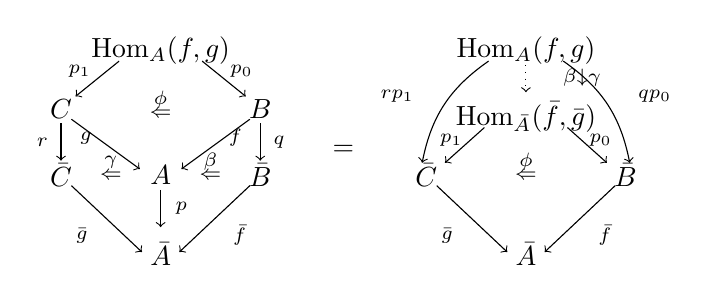
\begin{tikzpicture}[x=1.5em,y=1.5em]
  \node (hom) at (0,4.4) {$\mathrm{Hom}_A(f,g)$};
  \node (c) at (-2.4,3.0) {$C$};
  \node (b) at (2.4,3.0) {$B$};
  \draw[->] (-1.0,4.15) -- (-2.05,3.3);
  \node at (-1.95,3.9) {$\scriptstyle p_{1}$};
  \draw[->] (1.0,4.15) -- (2.05,3.3);
  \node at (1.95,3.9) {$\scriptstyle p_{0}$};
  \node at (0,3.22) {$\scriptstyle\phi$};
  \node at (0,2.88) {$\scriptstyle\Leftarrow$};
  \draw[->] (-2.4,2.65) -- (-2.4,1.75);
  \node at (-2.85,2.2) {$\scriptstyle r$};
  \draw[->] (2.4,2.65) -- (2.4,1.75);
  \node at (2.85,2.2) {$\scriptstyle q$};
  \draw[->] (-2.15,2.75) -- (-0.5,1.55);
  \node at (-1.8,2.3) {$\scriptstyle g$};
  \draw[->] (2.15,2.75) -- (0.5,1.55);
  \node at (1.8,2.3) {$\scriptstyle f$};
  \node (ab) at (0,1.4) {$A$};
  \node (cb) at (-2.4,1.4) {$\bar{C}$};
  \node (bb) at (2.4,1.4) {$\bar{B}$};
  \node at (-1.2,1.72) {$\scriptstyle\gamma$};
  \node at (-1.2,1.38) {$\scriptstyle\Leftarrow$};
  \node at (1.2,1.72) {$\scriptstyle\beta$};
  \node at (1.2,1.38) {$\scriptstyle\Leftarrow$};
  \draw[->] (0,1.05) -- (0,0.15);
  \node at (0.5,0.6) {$\scriptstyle p$};
  \node (abbar) at (0,-0.5) {$\bar{A}$};
  \draw[->] (-2.15,1.15) -- (-0.45,-0.45);
  \node at (-1.9,-0.05) {$\scriptstyle\bar{g}$};
  \draw[->] (2.15,1.15) -- (0.45,-0.45);
  \node at (1.9,-0.05) {$\scriptstyle\bar{f}$};
  \node at (4.4,2.0) {$=$};
  \begin{scope}[shift={(8.8,0)}]
  \node (hom) at (0,4.4) {$\mathrm{Hom}_A(f,g)$};
  \node (homb) at (0,2.8) {$\mathrm{Hom}_{\bar{A}}(\bar{f},\bar{g})$};
  \draw[->,dotted] (0,4.05) -- (0,3.4);
  \node at (1.35,3.75) {$\scriptstyle\beta\downarrow\gamma$};
  \draw[->] (-0.9,4.15) to[bend right=22] (-2.5,1.7);
  \node at (-3.1,3.3) {$\scriptstyle rp_{1}$};
  \draw[->] (0.9,4.15) to[bend left=22] (2.5,1.7);
  \node at (3.1,3.3) {$\scriptstyle qp_{0}$};
  \node (cb) at (-2.4,1.4) {$\bar{C}$};
  \node (bb) at (2.4,1.4) {$\bar{B}$};
  \draw[->] (-1.0,2.55) -- (-1.95,1.7);
  \node at (-1.8,2.25) {$\scriptstyle p_{1}$};
  \draw[->] (1.0,2.55) -- (1.95,1.7);
  \node at (1.8,2.25) {$\scriptstyle p_{0}$};
  \node at (0,1.72) {$\scriptstyle\phi$};
  \node at (0,1.38) {$\scriptstyle\Leftarrow$};
  \node (abbar) at (0,-0.5) {$\bar{A}$};
  \draw[->] (-2.15,1.15) -- (-0.45,-0.45);
  \node at (-1.9,-0.05) {$\scriptstyle\bar{g}$};
  \draw[->] (2.15,1.15) -- (0.45,-0.45);
  \node at (1.9,-0.05) {$\scriptstyle\bar{f}$};
  \end{scope}
\end{tikzpicture}
\end{center}
它在直至\trFiberedIsomorphism{}的意义下良定且函子（见%
\cref{ex:oplax-functoriality}）。
\end{observation}

\trCommaInfinityCategory{}的诸多用途之一，是定义一个\trInfinityCategory{} $A$ 的%
两个\trElement{}之间的内部\trMappingSpace{}。这正是我们采用记号「$\mathrm{Hom}_A$」的动机之一。

\begin{definition}[\trMappingSpace]\label{def:mapping-space}
\trInfinityCategory{} $A$ 的两个\trElement{} $x,y\colon\qcOne\to A$ 之间的%
\textbf{\trMappingSpace}（mapping space），是由如下拉回\trDiagram{}所定义的%
\trCommaInfinityCategory{} $\mathrm{Hom}_A(x,y)$
\begin{center}
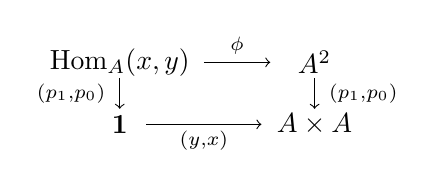
\begin{tikzpicture}[x=1.6em,y=1.6em]
  \node (tl) at (0,1.4) {$\mathrm{Hom}_A(x,y)$};
  \node (tr) at (4.4,1.4) {$A^{2}$};
  \node (bl) at (0,0) {$\qcOne$};
  \node (br) at (4.4,0) {$A\times A$};
  \draw[->] (1.9,1.4) -- (3.4,1.4);
  \node at (2.65,1.78) {$\scriptstyle\qcor{\phi}$};
  \draw[->] (0,1.05) -- (0,0.35);
  \node at (-1.1,0.7) {$\scriptstyle(p_{1},p_{0})$};
  \node at (0.48,0.78) {$\scriptstyle\lrcorner$};
  \draw[->] (4.4,1.05) -- (4.4,0.35);
  \node at (5.5,0.7) {$\scriptstyle(p_{1},p_{0})$};
  \draw[->] (0.6,0) -- (3.2,0);
  \node at (1.9,-0.38) {$\scriptstyle(y,x)$};
\end{tikzpicture}
\end{center}
\end{definition}

\trMappingSpace{}在定义 1.2.26 的意义下是\trDiscrete{}：

\begin{proposition}[\trMappingSpace{}是离散的]\label{prop:mapping-spaces-discrete}
对\trInfinityCategory{} $A$ 的任意一对\trElement{} $x,y\colon\qcOne\to A$，\trMappingSpace%
$\mathrm{Hom}_A(x,y)$ 是\trDiscrete{}。
\end{proposition}

\begin{proof}
我们必须证明：对任意\trInfinityCategory{} $X$，\trFunctorSpace{}%
$\mathrm{Fun}(X,\mathrm{Hom}_A(x,y))$ 是一个\trKanComplex{}。这恰好当%
$\mathrm{hFun}(X,\mathrm{Hom}_A(x,y))$ 是一个\trGroupoid{}时成立——也就是说，余定义域为%
$\mathrm{Hom}_A(x,y)$ 的任何 2-\trCell{}都是\trInvertible{}。由\trTwoCellConservativity{}，%
余定义域为 $\mathrm{Hom}_A(x,y)$ 的一个 2-\trCell{}是\trInvertible{}，恰好当它与%
\trIsofibration{} $(p_{1},p_{0})\colon\mathrm{Hom}_A(x,y)\twoheadrightarrow\qcOne\times\qcOne$%
的\trWhiskering{}复合是一条\trInvertible{} 2-\trCell{}；而事实上，由于 $\qcOne$ 是%
\trTwoTerminalObject{}，这一\trWhiskering{}复合是恒同。
\end{proof}

\cref{prop:comma-weak-universal-property}的弱\trUniversalProperty{}在 $C\times B$ 之上%
直至\trFiberedEquivalence{}（见\cref{def:fibered-equivalence}）刻画了诸\trCommaInfinityCategory{}。

\begin{proposition}[逗号∞-范畴的唯一性]\label{prop:comma-uniqueness}
对任何\trFiberedEquivalence{}于 $\mathrm{Hom}_A(f,g)\twoheadrightarrow C\times B$ 的%
\trIsofibration{} $(e_{1},e_{0})\colon E\twoheadrightarrow C\times B$，由\trEquivalence{}%
$e\colon E\rightleftarrows\mathrm{Hom}_A(f,g)$ 所编码的 2-\trCell
\begin{center}
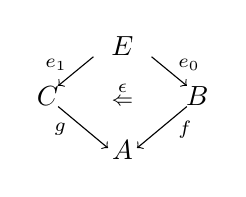
\begin{tikzpicture}[x=1.5em,y=1.5em]
  \node (e) at (0,2.0) {$E$};
  \node (c) at (-1.8,0.8) {$C$};
  \node (b) at (1.8,0.8) {$B$};
  \node (a) at (0,-0.5) {$A$};
  \draw[->] (-0.7,1.75) -- (-1.55,1.05);
  \node at (-1.6,1.55) {$\scriptstyle e_{1}$};
  \draw[->] (0.7,1.75) -- (1.55,1.05);
  \node at (1.6,1.55) {$\scriptstyle e_{0}$};
  \node at (0,1.0) {$\scriptstyle\epsilon$};
  \node at (0,0.66) {$\scriptstyle\Leftarrow$};
  \draw[->] (-1.55,0.55) -- (-0.35,-0.45);
  \node at (-1.5,0.0) {$\scriptstyle g$};
  \draw[->] (1.55,0.55) -- (0.35,-0.45);
  \node at (1.5,0.0) {$\scriptstyle f$};
\end{tikzpicture}
\end{center}
满足\cref{prop:comma-weak-universal-property}的弱\trUniversalProperty{}。反之，若%
$(d_{1},d_{0})\colon D\twoheadrightarrow C\times B$ 与 $(e_{1},e_{0})\colon E\twoheadrightarrow C\times B$%
配备有 2-\trCell
\begin{rveq}\label{eq:comma-uniqueness-cells}
\begin{tikzpicture}[x=1.5em,y=1.5em,baseline=(current bounding box.center)]
  \node (d) at (0,1.6) {$D$};
  \node (c) at (-1.8,0.4) {$C$};
  \node (b) at (1.8,0.4) {$B$};
  \node (a) at (0,-0.9) {$A$};
  \draw[->] (-0.7,1.35) -- (-1.55,0.65);
  \node at (-1.6,1.15) {$\scriptstyle d_{1}$};
  \draw[->] (0.7,1.35) -- (1.55,0.65);
  \node at (1.6,1.15) {$\scriptstyle d_{0}$};
  \node at (0,0.6) {$\scriptstyle\delta$};
  \node at (0,0.26) {$\scriptstyle\Leftarrow$};
  \draw[->] (-1.55,0.15) -- (-0.35,-0.85);
  \node at (-1.5,-0.5) {$\scriptstyle g$};
  \draw[->] (1.55,0.15) -- (0.35,-0.85);
  \node at (1.5,-0.5) {$\scriptstyle f$};
  \node at (4.0,0.4) {与};
  \begin{scope}[shift={(8.0,0)}]
  \node (e) at (0,1.6) {$E$};
  \node (c) at (-1.8,0.4) {$C$};
  \node (b) at (1.8,0.4) {$B$};
  \node (a) at (0,-0.9) {$A$};
  \draw[->] (-0.7,1.35) -- (-1.55,0.65);
  \node at (-1.6,1.15) {$\scriptstyle e_{1}$};
  \draw[->] (0.7,1.35) -- (1.55,0.65);
  \node at (1.6,1.15) {$\scriptstyle e_{0}$};
  \node at (0,0.6) {$\scriptstyle\epsilon$};
  \node at (0,0.26) {$\scriptstyle\Leftarrow$};
  \draw[->] (-1.55,0.15) -- (-0.35,-0.85);
  \node at (-1.5,-0.5) {$\scriptstyle g$};
  \draw[->] (1.55,0.15) -- (0.35,-0.85);
  \node at (1.5,-0.5) {$\scriptstyle f$};
  \end{scope}
\end{tikzpicture}
\end{rveq}
且它们满足\cref{prop:comma-weak-universal-property}的弱\trUniversalProperty{}，则%
$D\simeq_{C\times B}E$。
\end{proposition}

\begin{proof}
第一陈述的证明完全照搬\cref{prop:arrow-category-uniqueness}这一特殊情形的做法。我们证明逆方向，%
亦即给出练习 3.2.ii 的解。
考察满足\cref{prop:comma-weak-universal-property}所列诸弱\trUniversalProperty{}的%
一对 2-\trCell{} \eqref{eq:comma-uniqueness-cells}。\trOneCellInduction{}供给出%
一个\trSpan{}映射
\begin{center}
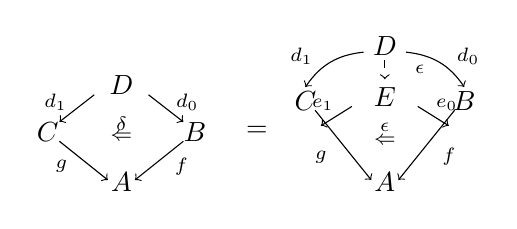
\begin{tikzpicture}[x=1.4em,y=1.4em]
  \node (d) at (0,1.8) {$D$};
  \node (c) at (-1.9,0.6) {$C$};
  \node (b) at (1.9,0.6) {$B$};
  \node (a) at (0,-0.7) {$A$};
  \draw[->] (-0.7,1.55) -- (-1.6,0.85);
  \node at (-1.7,1.35) {$\scriptstyle d_{1}$};
  \draw[->] (0.7,1.55) -- (1.6,0.85);
  \node at (1.7,1.35) {$\scriptstyle d_{0}$};
  \node at (0,0.8) {$\scriptstyle\delta$};
  \node at (0,0.46) {$\scriptstyle\Leftarrow$};
  \draw[->] (-1.6,0.35) -- (-0.35,-0.65);
  \node at (-1.55,-0.3) {$\scriptstyle g$};
  \draw[->] (1.6,0.35) -- (0.35,-0.65);
  \node at (1.55,-0.3) {$\scriptstyle f$};
  \node at (3.5,0.6) {$=$};
  \begin{scope}[shift={(6.8,0.8)}]
  \node (d) at (0,2.0) {$D$};
  \node (e) at (0,0.7) {$E$};
  \draw[->,dashed] (0,1.65) -- (0,1.15);
  \node at (0.9,1.4) {$\scriptstyle\qcor{\epsilon}$};
  \draw[->] (-0.55,1.85) to[bend right=25] (-2.05,0.95);
  \node at (-2.15,1.75) {$\scriptstyle d_{1}$};
  \draw[->] (0.55,1.85) to[bend left=25] (2.05,0.95);
  \node at (2.15,1.75) {$\scriptstyle d_{0}$};
  \node (c) at (-2.05,0.6) {$C$};
  \node (b) at (2.05,0.6) {$B$};
  \draw[->] (-0.85,0.45) -- (-1.65,-0.05);
  \node at (-1.6,0.5) {$\scriptstyle e_{1}$};
  \draw[->] (0.85,0.45) -- (1.65,-0.05);
  \node at (1.6,0.5) {$\scriptstyle e_{0}$};
  \node at (0,-0.1) {$\scriptstyle\epsilon$};
  \node at (0,-0.44) {$\scriptstyle\Leftarrow$};
  \node (a) at (0,-1.5) {$A$};
  \draw[->] (-1.8,0.35) -- (-0.35,-1.45);
  \node at (-1.65,-0.85) {$\scriptstyle g$};
  \draw[->] (1.8,0.35) -- (0.35,-1.45);
  \node at (1.65,-0.85) {$\scriptstyle f$};
  \end{scope}
\end{tikzpicture}
\end{center}
交换 $\delta$ 与 $\epsilon$ 的角色，便得到第二个\trSpan{}映射 $\qcor{\epsilon}\colon E\to D$，%
它具有性质 $\epsilon\qcor{\delta}\qcor{\epsilon}=\epsilon$ 与 $\delta\qcor{\epsilon}\qcor{\delta}=\delta$。%
\footnote{原书印作「$\epsilon'\qcor{\delta}\qcor{\epsilon}=\epsilon$」，其中 $\epsilon'$ 无定义，%
疑为「$\epsilon$」之误，此处径改。——译者注}%
由\cref{prop:whiskering-comma-bijection}可得：在 $C\times B$ 上%
$\qcor{\delta}\qcor{\epsilon}\cong\mathrm{id}_{E}$，在 $C\times B$ 上%
$\qcor{\epsilon}\qcor{\delta}\cong\mathrm{id}_{D}$。这就定义了一条\trFiberedEquivalence{}%
$D\simeq E$ 的数据。\footnote{正如警告 3.2.9 所暗示的那样，编码一条%
\trFiberedEquivalence{}的 2-范畴论数据存在一点轻微的含混。命题 3.6.4 为补全%
这一证明提供了一个小的助推。}
\end{proof}

沿我们处理\trArrowInfinityCategory{}时的同一约定，把「\trCommaInfinityCategory」%
这一称谓从\cref{def:comma-infinity-category}所构造的严格模型扩充到任何纤维化等价于%
它的\trInfinityCategory{}、并把其伴随的 2-\trCell{}称为「\trCommaCone」，是便利之举。例如，%
在 4.2 节中，我们将为一个由固定单纯集索引的\trDiagram{}之\trInfinityCategoryOfCones{}引入多个模型，%
它们在发展\trLimit{}的\trUniversalProperty{}的种种等价表述时很有用。

\subsection*{练习}

\begin{exercise}[命题 C.1.12]\label{ex:hom-p-factors}
通过观察 $\mathrm{Hom}_p(q,r)$ 分解为「$\partial\Delta[1]\hookrightarrow\Delta[1]$ 与 $p$ 的%
\trLeibnizCotensor」的一个\trPullback{}、再接上 $r\times q$ 的一个\trPullback{}来分解，%
完成\cref{prop:maps-between-commas}的证明。
\end{exercise}

\begin{exercise}\label{ex:oplax-functoriality}
利用\cref{prop:whiskering-comma-bijection}，为\cref{obs:oplax-cospan-maps}所描述的%
逗号构造在\trCospan{}的反松弛态射之下直至同构的函子性提供论证。
\end{exercise}

\begin{exercise}\label{ex:rectification}
\cref{ex:hom-p-factors}与\cref{ex:oplax-functoriality}例示了%
\trCommaInfinityCategory{}构造的严格单纯\trUniversalProperty{}与\trBicategory%
\trUniversalProperty{}各自的相对优点与缺点：前者给出一个严格函子的作用，却只对%
严格交换的\trCospan{}映射如此；后者给出\trCospan{}的反松弛变换的一个作用，%
却直至同构才是函子的。在这两种构造之间居中调停，用引理 1.2.19 与命题 1.4.9 把%
一个拟交换\trDiagram
\begin{center}
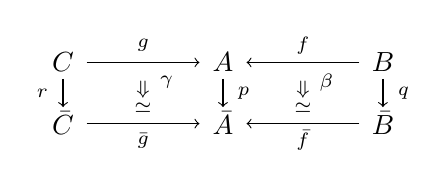
\begin{tikzpicture}[x=1.7em,y=1.7em]
  \node (c) at (0,1.3) {$C$};
  \node (a) at (3.4,1.3) {$A$};
  \node (b) at (6.8,1.3) {$B$};
  \node (cb) at (0,0) {$\bar{C}$};
  \node (ab) at (3.4,0) {$\bar{A}$};
  \node (bb) at (6.8,0) {$\bar{B}$};
  \draw[->] (0.5,1.3) -- (2.9,1.3);
  \node at (1.7,1.66) {$\scriptstyle g$};
  \draw[->] (6.3,1.3) -- (3.9,1.3);
  \node at (5.1,1.66) {$\scriptstyle f$};
  \draw[->] (0.5,0) -- (2.9,0);
  \node at (1.7,-0.36) {$\scriptstyle\bar{g}$};
  \draw[->] (6.3,0) -- (3.9,0);
  \node at (5.1,-0.36) {$\scriptstyle\bar{f}$};
  \draw[->] (0,0.95) -- (0,0.35);
  \node at (-0.44,0.65) {$\scriptstyle r$};
  \draw[->] (3.4,0.95) -- (3.4,0.35);
  \node at (3.84,0.65) {$\scriptstyle p$};
  \draw[->] (6.8,0.95) -- (6.8,0.35);
  \node at (7.24,0.65) {$\scriptstyle q$};
  \node at (1.7,0.72) {$\scriptstyle\Downarrow$};
  \node at (2.2,0.88) {$\scriptstyle\gamma$};
  \node at (1.7,0.34) {$\scriptstyle\simeq$};
  \node at (5.1,0.72) {$\scriptstyle\Downarrow$};
  \node at (5.6,0.88) {$\scriptstyle\beta$};
  \node at (5.1,0.34) {$\scriptstyle\simeq$};
\end{tikzpicture}
\end{center}
\trRectify{}成一个与之等价的严格交换\trDiagram{}，并证明诱导映射 $\mathrm{Hom}_p(q,r)$ 等价于%
$\beta\downarrow\gamma$。
\end{exercise}

\begin{exercise}\label{ex:oplax-equivalence}
证明：由如下\trDiagram
\begin{center}
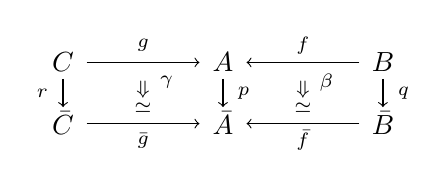
\begin{tikzpicture}[x=1.7em,y=1.7em]
  \node (c) at (0,1.3) {$C$};
  \node (a) at (3.4,1.3) {$A$};
  \node (b) at (6.8,1.3) {$B$};
  \node (cb) at (0,0) {$\bar{C}$};
  \node (ab) at (3.4,0) {$\bar{A}$};
  \node (bb) at (6.8,0) {$\bar{B}$};
  \draw[->] (0.5,1.3) -- (2.9,1.3);
  \node at (1.7,1.66) {$\scriptstyle g$};
  \draw[->] (6.3,1.3) -- (3.9,1.3);
  \node at (5.1,1.66) {$\scriptstyle f$};
  \draw[->] (0.5,0) -- (2.9,0);
  \node at (1.7,-0.36) {$\scriptstyle\bar{g}$};
  \draw[->] (6.3,0) -- (3.9,0);
  \node at (5.1,-0.36) {$\scriptstyle\bar{f}$};
  \draw[->] (0,0.95) -- (0,0.35);
  \node at (-0.44,0.65) {$\scriptstyle r$};
  \draw[->] (3.4,0.95) -- (3.4,0.35);
  \node at (3.84,0.65) {$\scriptstyle p$};
  \draw[->] (6.8,0.95) -- (6.8,0.35);
  \node at (7.24,0.65) {$\scriptstyle q$};
  \node at (1.7,0.72) {$\scriptstyle\Downarrow$};
  \node at (2.2,0.88) {$\scriptstyle\gamma$};
  \node at (1.7,0.34) {$\scriptstyle\simeq$};
  \node at (5.1,0.72) {$\scriptstyle\Downarrow$};
  \node at (5.6,0.88) {$\scriptstyle\beta$};
  \node at (5.1,0.34) {$\scriptstyle\simeq$};
\end{tikzpicture}
\end{center}
——其中 $\beta$ 与 $\gamma$ 是\trIsomorphism{}，而 $p$、$q$ 与 $r$ 是\trEquivalence{}——%
所诱导的\trCommaInfinityCategory{}之间的\trFunctor{}，在 $r\times q$ 之上定义了%
一个\trEquivalence
\begin{center}
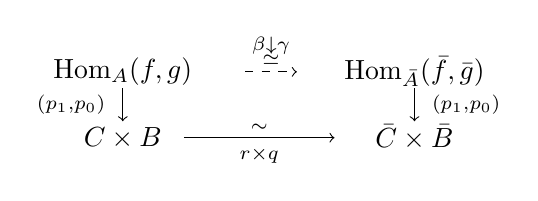
\begin{tikzpicture}[x=1.7em,y=1.7em]
  \node (tl) at (0,1.4) {$\mathrm{Hom}_A(f,g)$};
  \node (tr) at (6.2,1.4) {$\mathrm{Hom}_{\bar{A}}(\bar{f},\bar{g})$};
  \node (bl) at (0,0) {$C\times B$};
  \node (br) at (6.2,0) {$\bar{C}\times\bar{B}$};
  \draw[->,dashed] (2.6,1.4) -- (3.7,1.4);
  \node at (3.15,1.96) {$\scriptstyle\beta\downarrow\gamma$};
  \node at (3.15,1.66) {$\scriptstyle\simeq$};
  \draw[->] (0,1.05) -- (0,0.35);
  \node at (-1.1,0.7) {$\scriptstyle(p_{1},p_{0})$};
  \draw[->] (6.2,1.05) -- (6.2,0.35);
  \node at (7.3,0.7) {$\scriptstyle(p_{1},p_{0})$};
  \draw[->] (1.3,0) -- (4.5,0);
  \node at (2.9,0.22) {$\scriptstyle\sim$};
  \node at (2.9,-0.38) {$\scriptstyle r\times q$};
\end{tikzpicture}
\end{center}
\end{exercise}
